\documentclass[]{article}
\usepackage{amsmath}
%\usepackage{mhchem}
\usepackage{amssymb}
\usepackage{amsthm}
\usepackage{mathtools}
\usepackage{relsize}
\usepackage{algorithm}
\usepackage{algpseudocode}
\usepackage{tikz}
\usetikzlibrary{trees}
\usetikzlibrary{decorations.pathreplacing,calc}
\newcommand{\tikzmark}[1]{\tikz[overlay,remember picture] \node (#1) {};}

\newcommand*{\AddNote}[4]{%
	\begin{tikzpicture}[overlay, remember picture]
		\draw [decoration={brace,amplitude=0.5em},decorate,thick,black]
		($(#3)!(#1.north)!($(#3)-(0,1)$)$) --  
		($(#3)!(#2.south)!($(#3)-(0,1)$)$)
		node [align=center, text width=2.5cm, pos=0.5, anchor=west] {#4};
	\end{tikzpicture}
}%

%\usepackage{mathptmx,courier}
\usepackage[scaled=0.92]{helvet}
\normalfont
\usepackage{pifont,tabularx,varioref,url}
\usepackage[T1]{fontenc}
\DeclareMathOperator{\adj}{adj}
\DeclareMathOperator{\A}{\emph{\textbf{A}}}
\DeclareMathOperator{\B}{\emph{\textbf{B}}}
\input{structure.tex} % Include the file specifying the document structure and custom commands

%----------------------------------------------------------------------------------------
%	ASSIGNMENT INFORMATION
%----------------------------------------------------------------------------------------

% Required
\newcommand{\assignmentQuestionName}{P} % The word to be used as a prefix to question numbers; example alternatives: Problem, Exercise
%\newcommand{\assignmentClass}{} % Course/class
\newcommand{\assignmentTitle}{\text{ESO207-TA-1}} % Assignment title or name
\newcommand{\assignmentAuthorName}{Pathe Nevish Ashok (220757)} % Student name

% Optional (comment lines to remove)
%\newcommand{\assignmentClassInstructor}{ } % Intructor name/time/description
%\newcommand{\assignmentDueDate}{ } % Due date

\begin{document}
\begin{center}
	\Large ESO207 Theoretical Assignment 1
\end{center}
\section{Ideal profits}
\stuf{
		In the X world, companies have a hierarchical structure to form a large binary tree network (can be assumed to be a perfect binary tree). Thus every company has two sub companies as their children with the root as company X. The total number of companies in the structure is $N$. The wealth of each company follow the same general trend and doubles after every month. Also after every year, half of the wealth is distributed to the two child companies (i.e. one fourth to each) if they exist (i.e. the leaf
		node companies do not distribute their wealth). Given the initial wealth of each of the $N$ companies,
		you want to determine the final wealth of each company after m months.
		(A perfect binary tree is a special tree such that all leaf nodes are at the maximum depth of the tree,
		and the tree is completely filled with no gaps. Detailed explanation here
		}
\answer{
		\textbf{(a) Design an algorithm in $O(n^3 \log(m))$ complexity to find the final wealth of each company
		after m months.}
	}
	\stuf{
		\boxed{\texttt{Motivations:}}
		\begin{itemize}
			\item To get easier relation between parent and child company index $\to$ \textsc{Level-Order-Transversal}
			\item $n^3 log(m)$ factor suggests fast matrix exponentiation/multiplication similar to the \textsc{Clever-Fib-Algo} discussed in lectures
			\item We can easily form a recurrence relation between Wealth after $(k-1)$ years and $k$ years, thus suggesting matrix multiplication again
		\end{itemize}
		\hrule\vspace{4mm}
		
		First, we do a \textsc{Level-Order-Traversal} of the binary tree and store it in an array.\\
		For example, \textsc{Level-Order-Traversal} of the following tree gives the array $[W_1, W_2, W_3, W_4, W_5, W_6, W_7]$

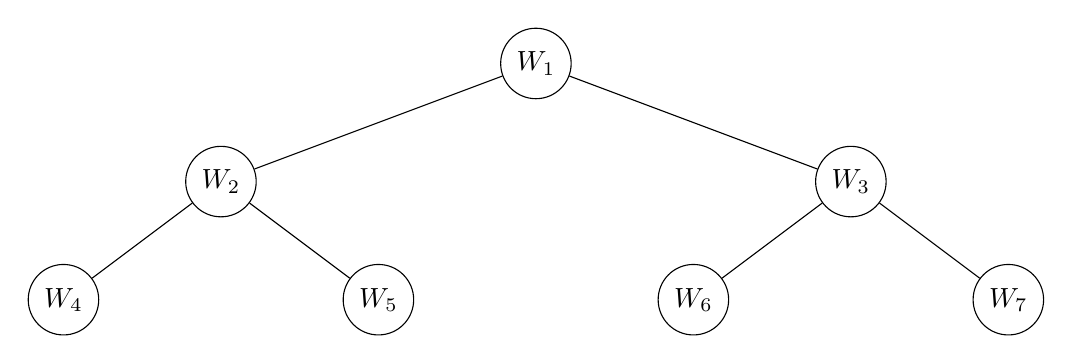
\begin{tikzpicture}[
	every node/.style = {minimum width = 1em, draw, circle},
	level/.style = {sibling distance = 80mm/#1},
	level 3/.style = {sibling distance = 20mm},
	level 4/.style = {sibling distance = 10mm}
	]
	\node {$W_1$}
	child {node {$W_2$} 
		child {node {$W_4$}
		}
		child {node {$W_5$}
		}
	}
	child {node {$W_3$}
		child {node {$W_6$}
		}
		child {node {$W_7$}
		}
	};
\end{tikzpicture}

		This allows us to find a relation between parent and child companies easily viz. $index(parent(j)) = \lfloor \frac{j}{2} \rfloor$
		We can keep track of the wealth of all companies after $k$ years as a $n\times 1$ matrix $W_k = \left[ W_{1,k}\ W_{2,k}\ W_{3,k}\ \cdots\ W_{n,k} \right]^T$\\
		We can represent the relation between $W_k$ and $W_{k-1}$ as follows:\\
		$
		\overset{W_k}{
		\begin{bmatrix}
			W_{1,k}\\ W_{2,k}\\ W_{3,k}\\ \vdots\\ W_{n,k}
		\end{bmatrix}}
		=
		\overbrace{
			2^{12}
		\begin{bmatrix}
			\frac{1}{2} & 0 & \cdots & 0\\
			\frac{1}{4} & \frac{1}{2} & \cdots & 0\\ 
			\vdots & \vdots & \ddots & \vdots\\ 
			0 & 0 & \cdots & 1
		\end{bmatrix}}^A
		\overset{W_{k-1}}{
		\begin{bmatrix}
				W_{1,k-1}\\ W_{2,k-1}\\ W_{3,k-1}\\ \vdots\\ W_{n,k-1}
		\end{bmatrix}
		}
		$
		
		Here, the matrix $A$ is constructed by setting $A[i][i] = 2^{11}$ and $A[i][\lfloor \frac{i}{2} \rfloor] = 2^{10}$ since after an year $W_{j,k} = 2^{12} \left(\frac{W_{\text{parent}(j),k-1}}{4} + \frac{W_{j,k-1}}{2}\right)$
		
		So, to find the wealth of companies after $m$ months, We first calculate $W_{j,\lfloor \frac{m}{12}\rfloor}$ and then the final answer $W'_{j,m} = 2^{m-12\lfloor \frac{m}{12}\rfloor} W_{j,\lfloor \frac{m}{12}\rfloor}$\\
		We accomplish this by using Matrix Exponentiation for finding powers of matrix $A$\\
		Finally, $W'_{j,m} = 2^{m-12\lfloor \frac{m}{12}\rfloor} A^{\lfloor \frac{m}{12}\rfloor} W_{j, 0}$\\	

		\boxed{\texttt{Pseudocode:}}
		\begin{algorithmic}
			\Function{Get-Wealth}{$BT, m$}
			\State $ogwealth \gets$ \Call{Level-Order-Traversal}{$BT$}
			\State $n \gets$ number of companies
			\State $A \gets [[0]]_{n\times n}$
			\For{$i$ from $0$ to $n-1$}
			\State $A[i][i] \gets 1/2 * 2^{12}$
			\If{$i \geq 2$}
			\State $A[i][\lfloor \frac{i}{2}\rfloor] \gets 1/4 * 2^{12}$
			\EndIf
			\If{$i > \lfloor \frac{n}{2} \rfloor$}
			\State $A[i][i] \gets 1 * 2^{12}$
			\EndIf
			\EndFor

			\State $A' \gets $\Call{matpow}{$n, A, \lfloor \frac{m}{12}\rfloor$}
			\State $H \gets $\Call{matpow}{$n, A', ogwealth$}
			\State $W' \gets [0]_m$
			\For{$i$ from $0$ to $n-1$}
				\State $W'[i] \gets W'[i] * 2^{(m \mod 12)}$
			\EndFor
			\State \textbf{return} $W'$ 
			
		\end{algorithmic}
				\dotfill
		\begin{algorithmic}
			\Function{Level-Order-Traversal}{$root$}
			\State $traversed \gets []$
			\If{$root$ is null}
			\State \textbf{return}
			\EndIf
			\State $queue \gets \text{Queue}()$ \Comment{Create an empty queue and enqueue the root node}
			\State $queue.\text{enqueue}(root)$
			\While{not $queue.\text{isEmpty}()$}
			\State $current\_node \gets queue.\text{dequeue}()$
			\State $traversed$.\Call{Append}{$current\_node.value$}
			\If{$current\_node.\text{left}$ is not null}
			\State $queue.\text{enqueue}(current\_node.\text{left})$
			\EndIf
			\If{$current\_node.\text{right}$ is not null}
			\State $queue.\text{enqueue}(current\_node.\text{right})$
			\EndIf
			\EndWhile
			
	\State \textbf{return} $traversed$ 
		\end{algorithmic}	
				\dotfill		
		\begin{algorithmic}
				\Function{kkk1}{$k$, $m_1$, $m_2$} \Comment{For matrix multiplication $(k\times k) \cdot (k\times 1)$}
				\State $m_3 \gets [0 \times k]$
				\For{$i$ from $0$ to $k-1$}
				\For{$j$ from $0$ to $k-1$}
				\State $m_3[i] \gets m_3[i] +  (m_1[i][j] * m_2[j])$
				\EndFor
				\EndFor
				\State \textbf{return} $m_3$
			\end{algorithmic}
		\dotfill
			\begin{algorithmic}
				\Function{kkkk}{$k$, $m1$, $m2$} \Comment{For matrix multiplication $(k\times k) \cdot (k\times k)$}
				\State $m_3 \gets [[0]]_{k\times k}$
				\For{$i$ from $0$ to $k-1$}
				\For{$j$ from $0$ to $k-1$}
				\State $m_3[i][j] \gets 0$
				\For{$m$ from $0$ to $k-1$}
				\State $m_3[i][j] \gets m_3[i][j] + (m_1[i][m] * m_2[m][j])$
				\EndFor
				\EndFor
				\EndFor
				\State \textbf{return} $m_3$
			\end{algorithmic}
				\dotfill
			\begin{algorithmic}
				\Function{matpow}{$k$, $base$, $pow$} \Comment{For matrix exponentiation}
				\State $mull \gets [[0]]_{k\times k}$
				\If{$pow = 1$}
				\For{$i$ from $0$ to $k-1$}
				\For{$j$ from $0$ to $k-1$}
				\State $mull[i][j] \gets base[i][j]$
				\EndFor
				\EndFor
				\State \textbf{return} $mull$
				\EndIf
				\State $temp \gets$ \Call{matpow}{$k$, $base$, $pow / 2$}
				\State $mull \gets$ \Call{kkkk}{$k$, $temp$, $temp$} \Comment{$O(n^3)$}
				\If{$pow \mod 2 = 1$}
				\State $mull \gets$ \Call{kkkk}{$k$, $mull$, $base$}
				\EndIf
				\State \textbf{return} $mull$
			\end{algorithmic}
		
		
}
		\answer{
		\textbf{(b) Analyze the time complexity of your algorithm and briefly argue about the correctness
			of your solution}
		}
		\stuf{
			\boxed{\texttt{Time Complexity Analysis :}}
			\begin{algorithmic}
				\Function{Get-Wealth}{$BT, m$}
				\State $ogwealth \gets$ \Call{Level-Order-Traversal}{$BT$} \Comment{Since each node is visited exactly once, $O(n)$}
				\State $n \gets$ number of companies \tikzmark{t1}
				\State $A \gets [[0]]_{n\times n}$ \tikzmark{b1}
				\For{$i$ from $0$ to $n-1$} \tikzmark{t2}
				\State $A[i][i] \gets 1/2 * 2^{12}$
				\If{$i \geq 2$}
				\State $A[i][\lfloor \frac{i}{2}\rfloor] \gets 1/4 * 2^{12}$
				\EndIf
			\If{$i > \lfloor \frac{n}{2} \rfloor$}
\State $A[i][i] \gets 1 * 2^{12}$
\EndIf
				\EndFor \tikzmark{b2}
				
				\State $A' \gets $\Call{matpow}{$n, A, \lfloor \frac{m}{12}\rfloor$} \Comment{$O(n^3 log(m))$}
				\State $H \gets $\Call{matpow}{$n, A', ogwealth$} \tikzmark{r1} \Comment{$O(n^3)$}
				\State $W' \gets [0]_m$
				\For{$i$ from $0$ to $n-1$}\tikzmark{t3}
				\State $W'[i] \gets W'[i] * 2^{(m \mod 12)}$
				\EndFor\tikzmark{b3}
				\State \textbf{return} $W'$ 
				
			\end{algorithmic}
			\\
			So, the overall time complexity of \textsc{Get-Wealth}$(BT,m)$ ia $T(n) = O(n) + O(1) + O(n) + O(n^3 log(m)) + O(n^3) + O(n) = O(n^3 log(m))$ (being the dominant term)\\
			
			The function \textsc{matpow}$(k, base, pow/2)$ gets called for $log(m)$ times i.e. until $pow/2$ reaches $1$ and inside each call of the function, we have the function \textsc{kkkk}$(k,temp, temp)$ being called for matrix multiplication, and it has three nested loops contributing $O(n^3)$ to the time complexity. Thus overall time complexity contribution of \textsc{matpow} is $O(n^3 \times log(m))$\\
			
			\boxed{\texttt{Correctness :}}\\
			We make the assertion that at end of $k-1$ years, we know the wealth of each company as $W_{k-1} = \left[ W_{1,{k-1}}\ W_{2,{k-1}}\ W_{3,{k-1}}\ \cdots\ W_{n,{k-1}} \right]^T$. Since after each month, the wealth doubles, so after an year we have $W_{j, k} = 2^{12} W_{j,k-1}$ (before distribution). Now, we distribute the wealth such that $W_{j, k} = 2^{12} \left(\frac{W_{\text{parent}(j),k-1}}{4} + \frac{W_{j,k-1}}{2}\right)$ since wealth of the company halves and then it inherits $1/4 ^{th}$ from its parent company. (Except for the companies at the bottom-most level of tree whose wealth doesn't halve) Now, to account for $m$ months, we have $k = \lfloor \frac{m}{12}\rfloor$ and the wealths of companies doubles for the leftover $m\mod 12$ months, So finally we have $W'_{j,m} = 2^{(m\mod 12)} W_{j,\lfloor \frac{m}{12}\rfloor}$
		}
		\answer{
		\textbf{(c) Consider the case of a single company (i.e. only root) in the tree. Give a constant time
			solution to find the final wealth after m months.}
		}
		\stuf{
			Considering the initial wealth to be $W_0$, since the root itself is the only company, it's wealth does not get distributed after every year. \\$\implies$ The company's wealth after $m$ months, $W_m = 2^m W_0$\\
			We can utilise binary-shift operators for getting an $O(1)$ solution\\
			\boxed{\texttt{W\_{j,m} = (W\_{j,0} << m)}}
		}
	

\newpage

\section{Moody Friends}
\stuf{
	$P$ friends arrive at a hotel after a long journey and want rooms for a night. This hotel has $n$ rooms
	linearly arranged in form of an array from left to right where array values depict the capacities of the
	rooms. As these are very close friends they will only consider consecutive rooms for staying. As you are
	the manager of the hotel you are required to find cheapest room allocation possible for them (sum of
	the capacities of selected rooms should be greater than or equal to $P$). Cost of booking every room is
	same and is equal to $C$.
}
\answer{
	\textbf{(a) Design an algorithm in $O(n)$ time complexity for determining the minimum cost
		room allocation. The allocated rooms should be consecutive in the array and their capacities should
		sum to atleast $P$.}
	}
	\stuf{
		\boxed{\texttt{Motivations:}}
		\begin{itemize}
			\item $O(n)$ suggests that we may need to process each element atmost a constant number of times
			\item This problems draws heavy similarity from the minimum sum subarray problem
		\end{itemize}
		\hrule\vspace{4mm}
		We can keep two pointers to keep track of the two ends of the subarray. Now, while we traverse the original array from left to right, at each step we check whether the sum achieved is greater than or equal to $P$, if yes then we remove the left most element of subarray (incrementing left pointer by 1) and continue the search for an even smaller length, and if not then we add take more elements in the subarray (incrementing right pointer by 1) and repeat this again.\\\\
\boxed{\texttt{Pseudocode:}}
\begin{algorithmic}
	\Function{Get-Minimum-Cost}{$rooms$}
	\State $l \gets 0$ \tikzmark{t1}
	\State $cost \gets \inf$
	\State $cap \gets 0$\tikzmark{b1}
	\For{$i\gets 0 \textbf{ to } n-1$}\tikzmark{t2}
		\State $cap \gets cap + rooms[i]$
		\While{$cap >= P$}
			\State $cost \gets \min(cost, i+1-l)$\tikzmark{r1}
			\State $cap \gets cap - rooms[l]$
			\State $l \gets l + 1$
		\EndWhile
	\EndFor  \tikzmark{b2}
	
	\State \textbf{return} $(cost * C)$ 
	
\end{algorithmic}
		\AddNote{t1}{b1}{r1}{$O(1)$}
		\AddNote{t2}{b2}{r1}{$O(n)$}
	}
	\answer{
	\textbf{(b)  Now suppose they don’t care about the cost and total capacity anymore. But they came up with a beauty criteria for an allocation. According to them, an allocation is beautiful if
		GCD (Greatest Common Divisor) of capacities of all rooms in the allocation is at least equal to or
		greater than a constant $K$. And they want to take maximum number of contiguous rooms possible.
		Your task is to design an algorithm in $O(nlog(n))$ time complexity for determining the maximum
		number of contiguous rooms they can get which satisfy the beauty constraints. You can assume
		access to a blackbox GCD algorithm which can give you GCD of two numbers in constant $O(1)$
		time.}
	}
	\stuf{
		\boxed{\texttt{Motivations:}}
		\begin{itemize}
			\item We can translate this problem as finding the maximum length of subarray such that "range-GCD" satisfies the given constraint
			\item Thus, thinking similar on the lines of Range-Minima problem, we construct a new data structure of size $n log(n)$
			\item We can effectively divide the problem in two parts:
			\begin{enumerate}
				\item Efficiently finding the range-GCD of a given range
				\item Efficiently finding the maximal length of such valid subarray
			\end{enumerate}
		\end{itemize}
		\hrule\vspace{4mm}
		We can use an $n \times log(n)$ matrix $S$ where $S[i][j]$ stores GCD of the range $A[i], A[i+1], ..., A[i+2^j]$ where $A$ is the original array. We can then binary search on the length of subarray such that range-GCD $>= K$ (Since if range-GCD $>= K$ for a subarray of length $m$ then it is valid for all lengths $<=m$ while after a maximal length, it won't be valid for all lengths $>$ maximal\_length)\\\\
		\boxed{\texttt{Pseudocode:}}
		\begin{algorithmic}
			\Function{Build-Matrix}{$rooms$}
			\State $n \gets $ number of rooms
			\State $log \gets [0]_{n+1}$
			\For{$i \gets 2$ \textbf{to} $n+1$}
			\State $log[i] \gets log[\lfloor \frac{i}{2}\rfloor] + 1$
			\EndFor
			\State $st \gets [[0]]_{n \times (log[n] + 1)}$
			\For{$i \gets 0$ \textbf{to} $n$}
			\State $st[i][0] \gets rooms[i]$
			\EndFor
			\For{$j \gets 1$ \textbf{to} $log[n]+1$}
			\For{$i \gets 0$ \textbf{to} $n - 2^j + 1$}
			\State $st[i][j] \gets \text{GCD}(st[i][j-1], st[i + 2^{j-1}][j-1])$
			\EndFor
			\EndFor
			\State \textbf{return} $st$
		\end{algorithmic}
				\dotfill
		\begin{algorithmic}
			\Function{Get-Range-GCD}{$st, L, R$}
			\State $k \gets$ \text{largest power of 2 such that} $2^k \leq R - L + 1$
			\State \textbf{return} $\text{GCD}(st[L][k], st[R - 2^k + 1][k])$
		\end{algorithmic}
				\dotfill
		\begin{algorithmic}
			\Function{Check-Length}{$arr, K, length$}
			\State $n \gets $ number of rooms
			\For{$i \gets 0$ \textbf{to} $n - length$}
			\If{\Call{Get-Range-GCD}{$st, i, i + length - 1$} $\geq K$}
			\State \textbf{return} \textbf{true}
			\EndIf
			\EndFor
			\State \textbf{return} \textbf{false}
		\end{algorithmic}
		\dotfill
		\begin{algorithmic}
			\Function{Get-Max-Length}{$rooms$}
				\State $n \gets$ \text{length of} $arr$
				\State $l \gets 0$
				\State $r \gets n$
				\State $maxLen \gets -1$
				
				\While{$l \leq r$}
				\State $mid \gets \lfloor \frac{l + r}{2} \rfloor$
				\If{\Call{Check-Length}{$arr, K, mid$}}
				\State $maxLen \gets mid$
				\State $l \gets mid + 1$
				\Else
				\State $r \gets mid - 1$
				\EndIf
				\EndWhile
				
				\State \textbf{return} $maxLen$
				\EndProcedure
			\end{algorithmic}
			
		
	}
		\answer{\textbf{(c) Give proof of correctness and time complexity analysis of your approach for part (a)}
	}
	\stuf{
		\boxed{\texttt{Proof of Correctness :}}\\
		We have two pointers, the range contained by them are the rooms of interest. In each iteration, we check whether the target capacity has been reached or not. If it is not then we take into account the next room and continue this until we reach a point when total capacity $\ge P$, after which we start removing rooms from the left and hence decreasing the length of our subarray. \\
		Our \textsc{Invariant} in this case is that at all times the $cost$ variable stores the sum of capacities of rooms between the two pointers i.e. it considers a valid subarray at all points of time.\\
		Also, Correctness is assured in both the cases:
		\begin{itemize}
			\item When the target capacity is not reached, we add more rooms to the subarray. This is valid since we are attempting to increase the sum.
			\item When the target capacity is already reached, we start removing rooms from the left to potentially reduce the subarray length and thus minimize the cost.
		\end{itemize} 
		In all the possible cases (i.e. with $cap >= P$), our algorithm explores all possible lengths of subarray and then finds the minimum length. Hence, it correctly finds the required minimum cost.\\\\
		\boxed{\texttt{Time Complexity Analysis:}}\\
		Each pointer can visit an element atmost once, and thus all the elements are processed atmost twice (initially adding it to the subarray for reaching target sum and then maybe removing it to minimize the length). Thus total time complexity $T(n) = 3 + n + cn + k = O(n), c, k$ being some constants
	}
}

\newpage

\section{BST universe}
\stuf{
You live in a BST world where people are crazy about collecting BSTs and trading them for high values.
You also love Binary Search Trees and possess a BST. The number of nodes in your BST is $n$.
}
\answer{
	\textbf{(a)  The Rival group broke into your lab to steal your BST but you were able to stop them.
		But still they managed to swap exactly two of the vertices in your BST. Design an $O(n)$ algorithm
		to find which nodes are swapped and the list of their common ancestors.}
	}
		
		
	\stuf{
		\boxed{\texttt{Motivations:}}
		\begin{itemize}
			\item In a normal BST, \textsc{Inorder-Traversal} gives us the sorted nodes
			\item While searching the nodes in the BST, we can take note of the nodes visited to know about their ancestors
		\end{itemize}
		\hrule\vspace{4mm}
		If the vertices weren't swapped, then, after traversing the tree using \textsc{Inorder-Traversal} algorithm, we'd get all the $n$ nodes in a sorted fashion. So, traversing using the same algorithm and then traversing through the sorted list, we can easily detect the two swapped vertices.\\\\
\boxed{\texttt{Pseudocode:}}
		\begin{algorithmic}
			\State $traversed \gets []$
			\Function{Inorder-Traversal}{$BST, node$} \Comment{Takes $O(n)$ time since each node is processed atmost once and processing takes constant time.}
			\If{$node <> \text{NULL}$}
			\State	\Call{Inorder-Traversal}{$BST$, $node.left$}
			\State $traversed$.\Call{Append}{$node.value$}
\State \Call{Inorder-Traversal}{$BST$, $node.right$}
			\EndIf 
			\State \textbf{return} $traversed$ 
			
		\end{algorithmic}
		
		\begin{algorithmic}
			\Function{Find-Swap}{$sorted$}
			\State $p, q \gets \text{NULL}$
			\For{$i\gets 0 \textbf{ to } n-2$}  
				\If{$sorted[i] > sorted[i+1]$}
					\State $p \gets sorted[i]$
					\State \textbf{break}
				\EndIf
				
			\EndFor
			\For{$i\gets n-1,1$}  
			\If{$sorted[i-1] > sorted[i]$}
			\State $q \gets sorted[i]$
			\State \textbf{break}
			\EndIf
			\EndFor
			\State \textbf{return} $m, n$ 
		\end{algorithmic}
	
		Thus, we obtain $m, n$ (the swapped vertices) in $O(n)$ time. (Since each node gets processed atmost once)
		Now, to get the list of common ancestors, we can search the vertices $m ,n$ in the (original, with vertices not swapped) BST and generate the list of nodes we visit on our way to search them respectively. We do this by searching the swapped vertices in modified BST and then swap them again. We then compare and take the common elements to get our list of common ancestors.\\\\
		\boxed{\texttt{Pseudocode:}}
			\begin{algorithmic}
				\Function{Get-Common-Ancestors}{$m, n, common$}
				\State $m\_ancestors \gets []$
				\State $n\_ancestors \gets []$
				\State $common \gets []$
				\State \Call{Search-N-Swap}{$BST, m, n$} \Comment{Search for $m$ and $n$ and then swap them}
				\State \Call{Search}{$BST, m, m\_ancestors$}
				\State \Call{Search}{$BST, n, n\_ancestors$}
				\State $i\gets 0$
				\While{$m\_ancestors[i] = n\_ancestors[i]$}
				\State $common$.\Call{Append}{$m\_ancestors[i]$}
			\end{algorithmic}
			\begin{algorithmic}
				\Function{Search}{$node, target, ancestors$}
				 \If{$node$ is \text{NULL}}
				\State \Return \text{NULL} 
				\EndIf
				\State $ancestors$.\Call{Append}{$node.value$}
				\If{$node.value$ = $target$}
				\State \Return $node$
				\EndIf
				\If{$target < node.value$}
				\State \Return \Call{Search}{$node.left, target, ancestors$}
				\Else
				\State \Return \Call{Search}{$node.right, target, ancestors$}
				\EndIf
			\end{algorithmic}
	Thus, we obtain the list of all common ancestors in the array $common$
	}
	\answer{
	\textbf{(b)  Seeing you were able to easily revert the damage to your tree, they attacked again
		and this time managed to rearrange exactly k of your nodes in such a way that none of the k
		nodes remain at the same position after the rearrangement. Also all the values inside this BST are
		upper bounded by a constant G. Your task is to determine the value of k and which nodes were
		rearranged. Design an algorithm of complexity $O(min( G + n, nlog(n) ))$ for the same.
		( Hint : Consider two cases for $G < nlog(n)$ and $G > nlog(n)$ )}
	}
	\stuf{
				\boxed{\texttt{Motivations:}}
		\begin{itemize}
			\item We use the hints to the fullest and obviously divide the problem into two cases
			\item $n log(n)$ (and even the part(a)) suggests sorting as a possible approach
			\item We use the same logic for second case
			\item For the first one, $O(G)$ part of the time complexity suggests some processing on a data structure of size of the order $G$
		\end{itemize}
		\hrule\vspace{4mm}
		We have two cases here:
		\begin{enumerate}
		\item $G < n log(n)$: Since, we have a cap on the range that the vertices can take, We can construct an array of length $G+1$ which contains the order in which they occur after \textsc{Inorder-Traversal} of the BST. Now, were the original BST preserved, the non-zero entries of our array would follow the increasing order of natural numbers $1, 2, ...$ i.e. $i+1$ at $i$'th index. Thus, we check for the indices where $arr[i] \ne (i+1)$ whose count gives us the number of rearranged vertices.\\
		In this case we have time complexity of $O(G + n)$\\\\
		\boxed{\texttt{Pseudocode:}}
		\begin{algorithmic}
			\Function{Find-Rearranged-Nodes-G}{$BST$}
			\State $traversed \gets []$
			\State $order \gets []$ 
			\State $rearranged\_nodes \gets []$
			\State \Call{Inorder-Traversal}{$BST$, $traversed$} 
			\For{$i\gets 0 \textbf{ to } n-1$} \Comment{$O(n)$}
				\State $order[traversed[i]+1] \gets i+1$
			\EndFor 
			\State $j \gets 1, k \gets 0$
			\For{$i\gets 1 \textbf{ to } G$} \Comment{$O(G)$}
			\If{$order[i] <> 0$}
				\If{$order[i] <> j$}
					\State $rearranged\_nodes$.\Call{Append}{$order[i]$}
					\State $k \gets k + 1$
				\EndIf
				\State $j \gets j + 1$
			\EndIf
			\EndFor 
	
			\State \textbf{return} $k, rearranged\_nodes$ 
		\end{algorithmic}
	
		 
		\item $G > n log(n)$: In this case, we can traverse the tree using \textsc{Inorder-Traversal} and then copy and sort the resulting array. Now we check for differences in the sorted and unsorted array, the count of which is exactly the number of rearranged vertices.\\
		In this case we have time complexity of $O(n log(n))$\\\\
		\boxed{\texttt{Pseudocode:}}
		\begin{algorithmic}
			\Function{Find-Rearranged-Nodes}{$BST$}
			\State $traversed \gets []$ 
			\State \Call{Inorder-Traversal}{$BST$, $traversed$} 
			\State $sorted \gets \Call{Copy-Array}{traversed}$
			\State \Call{sort}{$sorted$} \Comment{$O(n log(n))$}
			
			\State $rearranged\_nodes \gets []$ 
			\State $k, i \gets 0$ 
			\State $n = \Call{length}{traversed}$
			\While{$i < n$} 
			\If{$traversed[i] <> sorted[i]$} 
			\State $rearranged\_nodes$.\Call{Append}{$traversed[i]$}
			\State $k \gets k + 1$
			\EndIf
			
			\State $i \gets i + 1$
			\EndWhile
			
			\State \textbf{return} $k, rearranged\_nodes$ 
			\end{algorithmic}
		
		\end{enumerate}
		
	}

\newpage

\section{Helping Joker}
\stuf{
Joker was challenged by his master to solve a puzzle. His master showed him a deck of n cards. Each
card has value written on it. Master announced that all the cards are indexed from 1 to n from top to
bottom such that $(a_1 < a_2 < ... < a_{n−1} < a_n)$ .Then his master performed an operation on this 
invisible to Joker (Joker was not able to see what he did), he picked a random number k between 0 and
n and shifted the top k cards to the bottom of the deck. So after the operation arrangement of cards
from top to bottom looks like $(a_{k+1}, a_{k+2} . . . a_n, a_1, a_2 . . . a_k)$ where $(k + 1, k + 2 . . . n, 1, 2 . . . k)$ are
original indices in the sorted deck. Joker’s task is to determine the value of $k$. Joker can make a query
to his master. In a query, joker can ask to look at the value of any card in the deck. Joker asked you
for help because he knew you were taking an algorithms course this semester.
}
\answer{
	\textbf{(a) Design an algorithm of complexity $O(log(n))$ for Joker to find the value of $k$.}
}
	\stuf{
				\boxed{\texttt{Motivations:}}
		\begin{itemize}
			\item $log(n)$ is enough to suggest Binary Search (and also the partially sorted nature of the array)
		\end{itemize}
		\hrule\vspace{4mm}
		We can perform binary search on the value of $k$. We keep the initial range as $[0, n-1]$ and at each step we compare the values of the card at index $r$ and the card at index $mid =\lfloor \frac{l+r}{2} \rfloor$. Now, if
		\begin{enumerate}
			\item $a[mid] > a[r]$: This means that the smallest element is in the second half $[mid, r]$. So now, we set $l = mid + 1$ and continue the search
			\item $a[mid] < a[r]$: This means that the largest element lies in the first half $[l, mid]$. So we set $r = mid -1$ and continue
		\end{enumerate}
	We stop when the element at $mid$ is larger than that at $mid-1$ since we have found the smallest element. (We handle the edge case when $0$ cards are shifted to the bottom of the dark separately).\\\\
		\boxed{\texttt{Pseudocode:}}
	\begin{algorithmic}
		\Function{FindK}{$\text{deck}, n$}
%		\State $n \gets \text{length}(\text{deck})$\tikzmark{top}
%		\State $l \gets 0$
%		\State $r \gets n - 1$\tikzmark{bottom}
%		
%		\While{$l \leq r$} \Comment{iterates for $log_2(n)$ times}
%		\State $mid \gets \frac{l + r}{2}$
%		\State $a_1 \gets \text{query}(\text{deck}, 1)$  \Comment{Query for the value at index 1}
%		\State $a_{mid+1} \gets \text{query}(\text{deck}, mid)$ \tikzmark{right} \Comment{Query for the value at index $mid$}
%		
%		\If{$a_1 < a_{mid+1}$}
%		\State $l \gets mid + 1$
%		\Else
%		\State $r \gets mid - 1$
%		\EndIf
%		\EndWhile
%		\State \textbf{return} $l$
		\State 	\Comment{Here, \text{deck}$[i]$ means a query to master to get the value of $(i+1)^{th}$ card}
		\State $l \gets 0$ \tikzmark{t1}
		\State $r \gets n - 1$
		
		\If{$\text{deck}[l] \leq \text{deck}[r]$}
		\State \textbf{return} $l$
		\EndIf \tikzmark{b1}
		
		\While{$l \leq r$} \tikzmark{t2}
		\State $mid \gets \lfloor (l + r) / 2 \rfloor$
		\If{$\text{deck}[mid] < \text{deck}[mid-1]$} \tikzmark{r1}
		\State \textbf{return} $(n-mid)$
		\EndIf
		
		\If{$\text{deck}[mid] > \text{deck}[r]$}
		\State $l \gets mid + 1$
		\Else
		\State $r \gets mid - 1$ \tikzmark{b2}
	\end{algorithmic}
	\AddNote{t1}{b1}{r1}{$O(1)$}
	\AddNote{t2}{b2}{r1}{$O(log(n))$}

}
	\answer{
	\textbf{(b) Provide time complexity analysis for your strategy.}
}
	\stuf{
			We know that the initialisation steps take constant time while Binary Search takes $O(log(n))$ time since at every iteration the length of interval reduces by half. \\
			For binary search, we are basically cdeckying out 4-5 operations in each iteration. So the total time $T = \underset{log_2(n) \text{times}}{5 + 5 + \cdots + 5} = 5 log_2(n) = O(log(n))$\\
			Why $log_2(n)$ times?: At each iteration, length halves i.e. initial length $n$ reduces to $1$ in $k$ iterations, where $k$ can be given by $\frac{n}{2^k} = 1$ or $2^k = n \implies k = log_2(n)$\\
			Assuming the query time to be constant time, We have the final complexity of our algorithm as $O(1) + O(log(n)) + O(1) = O(log(n))$
	}



\newpage

\section{One Piece Treasure}
\stuf{
Strawhat Luffy and his crew got lost while searching for One piece (worlds largest known treasure). It
turns out he is trapped by his rival Blackbeard. In order to get out he just needs to solve a simple
problem. You being the smartest on his crew are summoned to help. On the gate out, you get to know
about a hidden string of lowercase english alphabets of length $n$. Also, an oracle is provided which
accepts an input query of format $(i, j)$, and returns true if the $substring(i, j)$ of the hidden string is a
palindrome and false otherwise in $O(1)$ time. But there is a catch, the place will collapse killing all the
crew members, if you ask any more than $n ∗ log^2
(n)$ queries to the oracle. The string is hidden and you
can’t access it. (Assume the string is very big i.e. $n$ is a large number)
}
\answer{
	\textbf{(a) You need to design a strategy to find number of palindromic substrings in the hidden
		string so your crew can safely escape from this region. Please state your algorithm clearly with
		pseudocode.
		(A contiguous portion of the string is called a substring)}
	}
	\stuf{
				\boxed{\texttt{Motivations:}}
		\begin{itemize}
			\item $n(log(n))^2$ doesn't really suggest anything but once we identify the predicate function here, it leads us to yet another Binary Search problem
			\item The trick is to deal with odd and even length palindromes differently and then binary search on possible length of palindromes
		\end{itemize}
		\hrule\vspace{4mm}
		We know that palindromes can be of two types; even-length and odd-length palindromes. We will handle them separately.\\
		For example, we define the center of the palindromes $b, aba, babab$ and radii $r$, in $a\ \overbrace{b\ a\ \underbrace{b}_{r = 0}\ a\ b}^{r=2} c$\\
		Thus, palindrome of length $d$ has radius $r = \lceil{\frac{d}{2}}\rceil - 1$\\
		Now, we can have $n$ centers of odd-length palindromes (since they can be single letters as well) and $n-1$ centers of even palindromes (counting $2$ consecutive elements)\\
		One important observation is that if we have a palindrome of radius $r$, then all strings with the same center and radii less than $r$ are palindrome i.e. If we define a predicate function \textsc{is-Palindrome}$(c, r)$ then we have a series of True's and then a series of False's. For the same reason, we can use binary search on the radii; for even and odd length palindromes differently.\\
		So, for even-length palindromes we query on $[c-r, c+r+2]$ (Since, actually the center consists of 2 elements) with radius ranging from $0$ to max possible from either end. Similarly, for odd-length, we query on $[c-r, c+r+1]$ for all possible radii.\\
		
		\boxed{\texttt{Pseudocode:}}
		\begin{algorithmic}
			\State 	\Comment{Here, \textsc{is-Palindrome}$(i,j)$ means a query to oracle to know if $substring(i,j)$ is a palindrome or not}
			\Function{Get-Number-of-Palindromes}{$string$}
			\State $pal \gets 0$
		
			\For{$c\gets 0 \textbf{ to } n-1$} \Comment{odd-length palindromes}
			\State $lo \gets 0$
			\State $hi \gets \min(c, n - c -1)$ \Comment{To ensure that the radius lies within the string from both ends}
			\While{$lo < hi$}
			\State $r \gets \lfloor \frac{l+r+1}{2}\rfloor$
			\If{\Call{is-Palindrome}{$c-r,c+r+1$}}
			\State $lo \gets r$
			\Else
			\State $hi = r - 1$
			\EndIf
			\State $pal \gets pal + l + 1$ \Comment{Since we assumed radius of single element to be 0}
			\EndWhile
			\EndFor  
		
			\For{$c\gets 0 \textbf{ to } n-2$} \Comment{even-length palindromes}
			\State $lo \gets -1$ \Comment{To include the case that two consecutive letters need not be palindrome}
			\State $hi \gets \min(c, n - c -2)$
			\While{$lo < hi$}
			\State $r \gets \lfloor \frac{l+r+1}{2}\rfloor$
			\If{\Call{is-Palindrome}{$c-r,c+r+2$}}
				\State $lo \gets r$
			\Else
				\State $hi = r - 1$
			\EndIf
			\State $pal \gets pal + l + 1$ \Comment{Since we assumed radius of empty string to be -1}
			\EndWhile
			\EndFor  
			
			\State \textbf{return} $pal$ 
		\end{algorithmic}
		Now, $pal$ gives us the total count of palindromes in the hidden string.\\
		Binary search requires $log(n)$ time complexity, so total complexity of the above algorithm becomes $O(n log(n)) < O(n (log(n))^2)$ and hence the place doesn't collapse!
	}





\end{document}